\documentclass[tikz]{standalone}
\usetikzlibrary{positioning, fit, arrows.meta, backgrounds}

\begin{document}
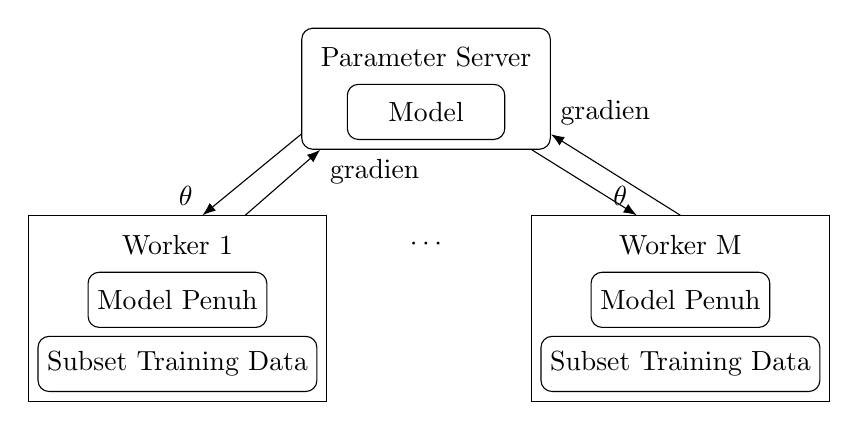
\begin{tikzpicture}[
    module/.style = {draw, rounded corners, minimum width = #1, minimum height = 7mm},
    module/.default=2cm,
    >=LaTeX
  ]

  \node[] (PStitle) {Parameter Server};
  \node[module, below=1mm of PStitle] (PSM) {Model};
  \node[fit=(PStitle) (PSM), module] (PS) {};
  \node[below=of PS] (Wcenter) {$\cdots$};

  \node[left=2cm of Wcenter] (W1) {Worker 1};
  \node[module, below=1mm of W1] (W1M) {Model Penuh};
  \node[module, below=1mm of W1M] (W1D) {Subset Training Data};
  \node[fit=(W1) (W1M) (W1D), draw] (W1C) {};

  \node[right=2cm of Wcenter] (WM) {Worker M};
  \node[module, below=1mm of WM] (WMM) {Model Penuh};
  \node[module, below=1mm of WMM] (WMD) {Subset Training Data};
  \node[fit=(WM) (WMM) (WMD), draw] (WMC) {};

  \draw[->] (PS.200) -- (W1C.75) node[anchor=south east] {$\theta$};
  \draw[->] (W1C.54) -- (PS.210) node[anchor=north west] {gradien};

  \draw[->] (PS.330) -- (WMC.115) node[anchor=south east]{$\theta$};
  \draw[->] (WMC.90) -- (PS.340) node[anchor=south west]{gradien};

\end{tikzpicture}
\end{document}
